\documentclass[11pt]{article}
\usepackage[scaled=0.92]{helvet}
\usepackage{geometry}
\geometry{letterpaper,tmargin=1in,bmargin=1in,lmargin=1in,rmargin=1in}
\usepackage[parfill]{parskip} % Activate to begin paragraphs with an empty line rather than an indent %\usepackage{graphicx}
\usepackage{amsmath,amssymb, mathrsfs, dsfont}
\usepackage{tabularx}
\usepackage[font=footnotesize,labelfont=bf]{caption}
\usepackage{graphicx}
\usepackage{xcolor}
%\usepackage[linkbordercolor ={1 1 1} ]{hyperref}
%\usepackage[sf]{titlesec}
\usepackage{natbib}
\usepackage{../../Tianpei_Report}
%\usepackage{appendix}
%\usepackage{algorithm}
%\usepackage{algorithmic}

%\renewcommand{\algorithmicrequire}{\textbf{Input:}}
%\renewcommand{\algorithmicensure}{\textbf{Output:}}



\begin{document}
\title{Lecture 5: Parameter Estimation in Graphical Models}
\author{ Tianpei Xie}
\date{Aug. 30th., 2022 }
\maketitle
\tableofcontents
\newpage
\allowdisplaybreaks
\section{Background knowledge}
Recall the formulation of Bayesian network and Markov network
\begin{itemize}
\item Given directed graph $\cG=(\cV, \cE)$, where $(s,t) \neq (t,s)$, the \textbf{directed graphical model}  factorizes the joint distribution into a set of \emph{factors} $\{p_s(x_s | x_{\pi(s)}): s\in \cV\}$ according to the ancestor relations defined in $\cG$
\begin{align}
p(x_1, \ldots, x_{m}) &= \prod_{s \in \cV}p_s(x_s | x_{\pi(s)}). \label{eqn: dag_graph_factorization}
\end{align} This class of models are also referred as \emph{\textbf{Bayesian networks}} \citep{koller2009probabilistic}.


\item Given undirected graph $\cG=(\cV, \cE)$, where $(s,t) = (t,s)$, the joint distribution of \textbf{Markov random fields} (\textbf{Markov network}) \emph{factorize} as
\begin{align}
p(x_1, \ldots, x_{m}) &= \frac{1}{Z}\prod_{C \in \cC}\psi_{C}(x_{C}),\label{eqn: mrf_graph_factorization}
\end{align} where $Z$ is a constant chosen to ensure that the distribution is normalized. The set $\cC$ is often taken to be the \emph{set of all \textbf{maximal cliques} of the graph}, i.e., the set of cliques that are \emph{not} properly contained within any other clique. Note that any representation based on nonmaximal cliques can always be converted to one based on maximal cliques by redefining the compatibility function on a maximal clique to be the \emph{product} over the compatibility functions on the \emph{subsets} of that clique.

\item The canonical representation of \underline{\emph{\textbf{exponential famlity}}} of distribution has the following form
\begin{align}
p(x_1, \ldots, x_{m}) = p(\mb{x}; \mb{\eta}) &= \exp\paren{\inn{\mb{\eta}}{\mb{\phi}(\mb{x})} - A(\mb{\eta})}h(\mb{x})\nu(d\mb{x}) \nonumber \\
&= \exp\paren{\sum_{\alpha}\eta_{\alpha}\phi_{\alpha}(\mb{x}) -  A(\mb{\eta})} \label{eqn: exp_fam}
\end{align} where $\phi$ is a feature map  and $\mb{\phi}(\mb{x})$ defines a set of \emph{\textbf{sufficient statistics}} (or \emph{\textbf{potential functions}}). The normalization factor is defined as
\begin{align*}
 A(\mb{\eta}) &:= \log \int \exp\paren{ \inn{\mb{\eta}}{\mb{\phi}(\mb{x})} }h(\mb{x})\nu(d\mb{x}) = \log Z(\mb{\eta})
\end{align*} $A(\mb{\eta})$ is also referred as \textbf{\emph{log-partition function}} or \emph{cumulant function}. The parameters $\mb{\eta} = (\eta_{\alpha})$ are called \textbf{\emph{natural parameters}}  or \emph{canonical parameters}. The canonical parameter $\set{\eta_{\alpha}}$ forms a \textbf{natural (canonical) parameter space}
\begin{align}
\Omega = \set{\mb{\eta} \in \bR^{d}: A(\mb{\eta}) < \infty} \label{eqn: canonical_space}
\end{align}

\item The exponential family is the unique solution of \textbf{\emph{maximum entropy estimation}} problem:
\begin{align}
\min_{q \in \Delta}&\quad \kl{q}{p_{0}} \label{eqn: max_ent}\\
\text{s.t.}&\quad \E{q}{\phi_{\alpha}(X)} = \mu_{\alpha}\,\quad  \forall\, \alpha \in \cI   \label{eqn: max_ent_mean_constraint}
\end{align} where $\kl{q}{p_0} = \int \log(\frac{q}{p_0}) q dx = \E{q}{\log\frac{q}{p_0}}$ is the relative entropy or the Kullback-Leibler divergence of $q$ w.r.t. $p_0$.

Here $\mb{\mu} = (\mu_{\alpha})_{\alpha \in \cI}$ is a set of  \textbf{\emph{mean parameters}}. The space of mean parameters $\cM$ is a \emph{convex polytope} spanned by potential functions $\set{\phi_{\alpha}}$.
\begin{align}
\cM &:= \set{\mb{\mu} \in \bR^d: \exists q\,\; \text{s.t. } \E{q}{\phi_{\alpha}(X)} = \mu_{\alpha}\,\quad  \forall\, \alpha \in \cI} = \text{conv}\set{\phi_{\alpha}(x),\; x\in \cX, \;\alpha \in \cI}  \label{eqn: marginal_polytope}
\end{align}

\item Note that $A(\mb{\eta})$ is a convex function and its gradient $\grad{}{A}: \Omega \rightarrow \cM^{\circ}$ is a bijection between the natural parameter space $\Omega$ and the \underline{\textbf{interior}} of $\cM$,  $\cM^{\circ}$; $\grad{}{A}(\mb{\eta}) = \mb{\mu}$ based on the following equation 
\begin{align}
\partdiff{A}{\eta_{\alpha}} &= \E{\mb{\eta}}{\phi_{\alpha}(X)} := \int_{\cX^{m}}\phi_{\alpha}(\mb{x}) q(\mb{x}; \mb{\eta}) d\mb{x} = \mu_{\alpha} \label{eqn: partition_first_order}
\end{align}

\item Moreover $A(\mb{\eta})$ has a variational form 
\begin{align}
A(\mb{\eta}) &=  \sup_{\mb{\mu} \in \cM}\set{ \inn{\mb{\eta}}{\mb{\mu}} - A^{*}(\mb{\mu})} \label{eqn: log_partition_variational_form}
\end{align}
where $A^{*}(\mb{\mu})$ is the conjugate dual function of $A$ and it is defined as
\begin{align}
A^{*}(\mb{\mu}) &:= \sup_{\mb{\eta} \in \Omega} \set{\inn{\mb{\mu}}{\mb{\eta}} - A(\mb{\eta})} \label{eqn: conjugate_dual_partition}
\end{align}

It is shown that $A^{*}(\mb{\mu})  = -H(q_{\mb{\eta}(\mb{\mu})})$ for $\mb{\mu} \in  \cM^{\circ}$ which is the negative entropy. $A^{*}(\mb{\mu})$ is also the optimal value for the \textbf{maximum likelihood estimation} problem on $p$. The exponential family can be reparameterized according to its mean parameters $\mb{\mu}$ via backward mapping $(\grad{}{A})^{-1}: \cM^{\circ} \rightarrow  \Omega$, called \textbf{mean parameterization}.

\item The maximum likelihood estimation of exponential family  is essentially the \underline{\textbf{dual problem}} of the maximum entropy estimation \eqref{eqn: max_ent}.
\begin{align}
\max_{\mb{\eta}} &\; \frac{1}{N}\sum_{n=1}^{N}\log q_{\mb{\eta}}(X_{n}) \nonumber\\
\Rightarrow \max_{\mb{\eta}}&\, \inn{\bar{\mb{\mu}}}{\mb{\eta}} - A(\mb{\eta}) \label{eqn: mle}
\end{align} where $\bar{\mb{\mu}} = \hat{\mathds{E}}_{}[\mb{\phi}(X)] = \frac{1}{N}\sum_{n=1}^{N}\mb{\phi}(X_{n})$ fits the moment matching conditions.  \eqref{eqn: mle} is the right-hand side of the conjugate dual of log-partition function $A^{*}$ in \eqref{eqn: conjugate_dual_partition}. Thus we have one statistical interpretation of this variational problem \eqref{eqn: conjugate_dual_partition}: $A^{*}$ is the \textbf{optimal value of the rescaled log likelihood} \eqref{eqn: mle}. 

Also see that the gradient of log-likelihood function 
\begin{align}
\grad{\mb{\eta}}{\frac{1}{N}\sum_{n=1}^{N}\log q_{\mb{\eta}}(X_{n}) }&= \grad{\mb{\eta}}{\paren{\inn{\hat{\mb{\mu}}}{\mb{\eta}} - A(\mb{\eta}) }} \nonumber\\
&=  \hat{\mathds{E}}_{}[\mb{\phi}(X)] - \E{\mb{\eta}}{\mb{\phi}(X)} \label{eqn: grad_log_likelihood}\\
&=  \hat{\mb{\mu}} - \mb{\mu}  = \text{sample mean} - \text{model mean}  \nonumber
\end{align} This gives the moment matching condition $\E{\mb{\eta}^{*}}{\mb{\phi}(X)} = \hat{\mb{\mu}}$ of MLE optimal solution $\mb{\eta}^{*}$.
From the formula above, whenever $\hat{\mb{\mu}} \in \cM^{\circ}$, there exists a \textbf{unique} maximum likelihood solution.



\item We can formulate the \textbf{KL divergence} between two distributions in exponential family $\Omega$ using its primal and dual form
\begin{itemize}
\item \textbf{Primal-form}: given $\mb{\eta}_1, \mb{\eta}_2 \in \Omega$
\begin{align}
\kl{p_{\mb{\eta}_1}}{p_{\mb{\eta}_2}} \equiv  \kl{\mb{\eta}_1}{\mb{\eta}_2}
&=  A(\mb{\eta}_2) - A(\mb{\eta}_1) -  \inn{\mb{\mu}_{1}}{\mb{\eta}_2 - \mb{\eta}_1}  \label{eqn: kl_primal}\\
&\equiv  A(\mb{\eta}_2) - A(\mb{\eta}_1) -  \inn{\grad{}{A}(\mb{\eta}_1)}{\mb{\eta}_2 - \mb{\eta}_1}  \nonumber
\end{align}

\item \textbf{Primal-dual form}: given $\mb{\mu}_1 \in \cM, \mb{\eta}_2 \in \Omega$
\begin{align}
 \kl{\mb{\mu}_1}{\mb{\eta}_2} &= A(\mb{\eta}_2) + A^{*}(\mb{\mu}_1) - \inn{\mb{\mu}_{1}}{\mb{\eta}_2}  \label{eqn: kl_primal_dual}
\end{align}

\item \textbf{Dual-form}: given $\mb{\mu}_1, \mb{\mu}_2  \in \cM$
\begin{align}
 \kl{\mb{\mu}_1}{\mb{\mu}_2} &= A^{*}(\mb{\mu}_1) - A^{*}(\mb{\mu}_{2}) - \inn{\mb{\eta}_2}{\mb{\mu}_{1} - \mb{\mu}_{2}}  \label{eqn: kl_dual} \\
 &\equiv  A^{*}(\mb{\mu}_1) - A^{*}(\mb{\mu}_{2}) - \inn{\grad{}{A^{*}}(\mb{\mu}_{2})}{\mb{\mu}_{1} - \mb{\mu}_{2}} \nonumber
\end{align}
\end{itemize}
\end{itemize}


\section{Parameter estimation in fully observed models}
The simplest case of parameter estimation corresponds to the case of fully observed data: a collection $\mb{X}^{1:n} := \{\mb{X}^1,\ldots, \mb{X}^n\}$ of $n$ independent
and identically distributed (i.i.d.) $m$-vectors, each sampled according to $p_{\mb{\eta}}$. Suppose that our goal to estimate the unknown parameter $\mb{\eta}$, which
we view as a deterministic but nonrandom quantity for the moment. This problem is solved via maximum likelihood estimation. For exponential family, the MLE can be formulated as in \eqref{eqn: mle},\ The optimal solution is \textbf{unique} and is specified by the \textbf{\emph{moment matching conditions}}.
\subsection{Maximum likelihood for triangulated graphs}
\begin{figure}
\begin{minipage}[t]{1\linewidth}
  \centering
  \centerline{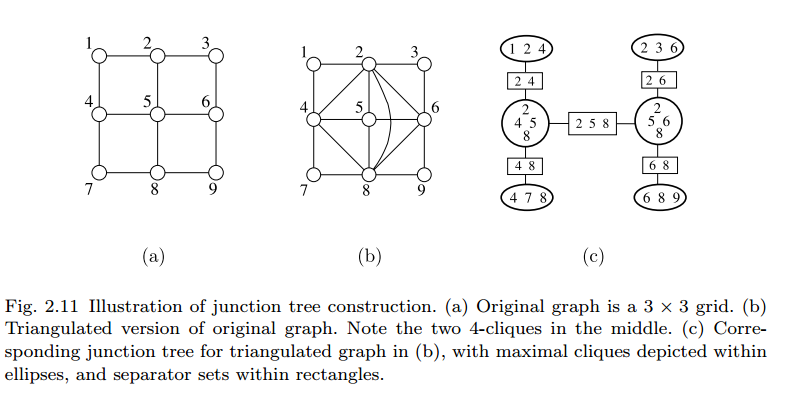
\includegraphics[scale = 0.5]{triangulation_junction_tree.png}}
\end{minipage}
\caption{\footnotesize{\textbf{Triangulation and junction tree. \citep{wainwright2008graphical}}}}
\label{fig: triangulation_junction_tree}
\end{figure}
In this section, we focus on solving the MLE problem \eqref{eqn: mle} on \emph{triangulated graphs}. We say that a graph is \underline{\emph{\textbf{triangulated}}} if every cycle of length \emph{four} or longer has a \emph{chord}, meaning an edge joining a pair of nodes that are not adjacent on the cycle. \textbf{A key \underline{theorem}} is that a graph $\cG$ has a \underline{\emph{\textbf{junction tree}}} if and only if it is triangulated. See Figure \ref{fig: triangulation_junction_tree} for an illustration. 

For triangulated graphs, the MLE can be written as a \emph{\textbf{closed-form function}} of the \emph{\textbf{empirical marginals}} $\mb{\mu}$ \citep{wainwright2008graphical}. For the sake of simplicity, let us consider the \emph{simplest} triangulated graph: a tree $\cT = (\cV, \cE)$ with discrete variables $\cX = \set{0,1,\ldots, r-1}$. Recall the pairwise Markov random field with indicator potentials
\begin{align}
\phi_{s;j}(x_s) &= \ind{x_s = j}  \label{eqn: metric_label_sufficient}
\end{align} 
Moreover, for each edge $(s,t)$ and pair of values $(j,k) \in \cX \times \cX$ , define the sufficient statistics
\begin{align}
\phi_{st;jk}(x_s, x_t) &= \ind{x_s = j \, \land x_{t} = k}  \label{eqn: metric_label_sufficient2}
\end{align}
The joint distribution is 
\begin{align}
p(x_1, \ldots, x_m; \mb{\eta}) &= \exp\paren{\sum_{s\in \cV}\sum_{j \in \cX}\eta_{s;j}\,\phi_{s;j}(x_s)  + \sum_{(s,t) \in \cE}\sum_{(j,k) \in \cX \times \cX}\eta_{st;jk}\,\phi_{st;jk}(x_s, x_t)  - A(\mb{\eta})}, \label{eqn: potts_model}
\end{align} The mean parameter space $\cM(\cG)$ is the \emph{\textbf{marginal polytope}} over $\cG$ since 
\begin{align*}
\cM(\cG) &:= \set{\mb{\mu} \in \bR^d: \exists q\,\; \text{s.t. } \E{q}{\phi_{\alpha}(X)} = \mu_{\alpha}\,\quad  \forall\, \alpha \in \cI} \\
\text{where }& \mu_{st;jk} = \bP_{\mb{\eta}}(X_s = j \land X_t = k), \quad \forall s,t, j, k \\
& \mu_{s;j} = \bP_{\mb{\eta}}(X_s = j ),  \quad \forall s, j
\end{align*} defines a set of matching constraints on the marginal distribution of $p$ within each factor.  

Given an i.i.d. sample $\mb{X}^{1:n} := \{\mb{X}^1,\ldots,\mb{X}^n\}$, the \emph{\textbf{empirical mean parameters}} correspond to the \underline{\textbf{singleton}} and \underline{\textbf{pairwise marginal probabilities}}:
\begin{align}
\hat{\mu}_{s;j} = \frac{1}{n}\sum_{i=1}^{n}\ind{X_{s}^{i} = j} \text{ and } \hat{\mu}_{st;jk} = \frac{1}{n}\sum_{i=1}^{n}\ind{X_s^{i} = j \, \land X_{t}^{i} = k} \label{eqn: emp_marginal}
\end{align} For this particular exponential family, our assumption that $\hat{\mb{\mu}} \in \cM^{\circ}$ means that the empirical marginals are all strictly \emph{positive}. 
Now choose $\hat{\mb{\eta}}$ as
\begin{align}
\hat{\eta}_{s,j} &= \log \hat{\mu}_{s;j}, \quad \forall s\in \cV, j \in \cX \label{eqn: mle_marginal_matching_single}\\
\hat{\eta}_{st;jk} &= \log \frac{ \hat{\mu}_{st;jk}}{\hat{\eta}_{s,j} \hat{\eta}_{t,k}}, \quad \forall (s,t) \in \cE, (j, k) \in \cX \times \cX. \label{eqn: mle_marginal_matching_pair}
\end{align} We now claim that $\hat{\mb{\eta}} = \hat{\mb{\eta}}_{mle}$ by proving that $\hat{\mb{\eta}}$ satisfies the moment matching conditions. Substituting \eqref{eqn: mle_marginal_matching_single} and \eqref{eqn: mle_marginal_matching_pair} into \eqref{eqn: potts_model},  the \underline{\textbf{joint distribution under}} $\hat{\mb{\eta}}$ is 
\begin{align}
p(x_1, \ldots, x_m; \hat{\mb{\eta}}) &=\prod_{s\in \cV}\hat{\mu}_{s}(x_s)\prod_{(s,t) \in \cE}\frac{\hat{\mu}_{s,t}(x_s, x_t)}{\hat{\mu}_{s}(x_s)\hat{\mu}_{t}(x_t)} \label{eqn: mle_joint_dist}
\end{align} Note that the log-partition function is $A(\hat{\mb{\eta}}) = 0$. Moreover, the distribution $p(\mb{x}; \hat{\mb{\eta}})$ has its \textbf{marginal distributions} as the empirical quantities $\hat{\mu}_{s}$ and $\hat{\mu}_{s,t}(x_s, x_t)$. To show this, we use an inductive "leaf-stripping" argument since by marginalize over leaf node variable. For example, for leaf node $u$, it only connects to one edge $(u,v)$, so averaging $p(\mb{x})$ over $x_u$ produces 
\begin{align*}
\sum_{x_u}p(x_1, \ldots, x_m; \hat{\mb{\eta}})&=\sum_{x_u}\hat{\mu}_{u}(x_u)\frac{\hat{\mu}_{u,v}(x_u, x_v)}{\hat{\mu}_{u}(x_u)\hat{\mu}_{v}(x_v)} \prod_{s\in \cV - \{u\}}\hat{\mu}_{s}(x_s)\prod_{(s,t) \in \cE - \{(u,v)\}}\frac{\hat{\mu}_{s,t}(x_s, x_t)}{\hat{\mu}_{s}(x_s)\hat{\mu}_{t}(x_t)}\\
&=\frac{ \sum_{x_u}\hat{\mu}_{u,v}(x_u, x_v)}{\hat{\mu}_{v}(x_v)} \prod_{s\in \cV - \{u\}}\hat{\mu}_{s}(x_s)\prod_{(s,t) \in \cE - \{(u,v)\}}\frac{\hat{\mu}_{s,t}(x_s, x_t)}{\hat{\mu}_{s}(x_s)\hat{\mu}_{t}(x_t)}\\
&= \prod_{s\in \cV - \{u\}}\hat{\mu}_{s}(x_s)\prod_{(s,t) \in \cE - \{(u,v)\}}\frac{\hat{\mu}_{s,t}(x_s, x_t)}{\hat{\mu}_{s}(x_s)\hat{\mu}_{t}(x_t)} := p(\mb{x}_{-u}; \cT_{-u})
\end{align*} And the result is of the same form on a tree $\cT_{-u} := (\cV - \{u\},  \cE - \{(u,v)\})$. Thus we can use induction to marginalize all other variables from leaf to root except for $x_s$ to obtain the result. \qed

Thus, we show that \textbf{tree-based model} $p(\mb{x}; \hat{\mb{\eta}})$ under maximum likelihood estimator $\hat{\mb{\eta}} = \hat{\mb{\eta}}_{mle}$ has an explicit closed-form expression \eqref{eqn: mle_joint_dist}. 

%\subsection{Iterative Methods for Computing MLEs}


\newpage
\section{Parameter estimation in partially observed models}
A more challenging version of parameter estimation arises in the partially observed setting, in which the random vector $\mb{X} \sim p_{\mb{\eta}}$ is not
observed directly, but \emph{indirectly} via a "noisy" version $\mb{Y}$ of $\mb{X}$. The \emph{\textbf{expectation-maximization (EM) algorithm}} provides a general approach to computing MLEs in this partially observed setting. 
\subsection{Exact EM algorithm in exponential families}
Suppose that the set of random variables is partitioned into a vector $\mb{Y}$ of observed variables, and a vector $\mb{X}$ of unobserved variables, and the
probability model is a \emph{joint exponential family} distribution for $(\mb{X},\mb{Y})$:
\begin{align}
p(\mb{x}, \mb{y}; \mb{\eta}) &= \exp\paren{\inn{\mb{\eta}}{\mb{\phi}(\mb{x}, \mb{y})} - A(\mb{\eta})} \label{eqn: latent_exp_joint}
\end{align} Given an observation $\mb{Y} = \mb{y}$, we can also form the conditional distribution
\begin{align}
p(\mb{x} | \mb{y},  \mb{\eta}) &= \frac{p(\mb{x}, \mb{y}; \mb{\eta})}{\int_{\mb{x}}p(\mb{x}, \mb{y}; \mb{\eta}) \nu(d\mb{x})} \nonumber \\
&:= \exp\paren{\inn{\mb{\eta}}{\mb{\phi}(\mb{x}, \mb{y})} - A_{\mb{y}}(\mb{\eta})} \label{eqn: latent_exp_conditional}
\end{align} where the log-partition for fixed $\mb{y}$ is given as 
\begin{align}
A_{\mb{y}}(\mb{\eta}) &= \log\int_{\mb{x} \in \cX^{m}} \exp\paren{\inn{\mb{\eta}}{\mb{\phi}(\mb{x}, \mb{y})}} \nu(d\mb{x})  \label{eqn: latent_log_partition}
\end{align} Note $\mb{\phi}(\cdot, \mb{y})$ for fixed $\mb{y}$ is function of latent variables $\mb{x}$.

The maximum likelihood estimation is for observed likelihood function on $\mb{Y}$, which is referred to as the \emph{\textbf{incomplete log likelihood}} in the setting of EM. This incomplete log likelihood is given by the integral
\begin{align}
\ell(\mb{\eta} ;\mb{y}) &=  \log\int_{\mb{x} \in \cX^{m}}\exp\paren{\inn{\mb{\eta}}{\mb{\phi}(\mb{x}, \mb{y})} - A(\mb{\eta})}\nu(d\mb{x})  \nonumber\\
&=\underline{A_{\mb{y}}(\mb{\eta})  - A(\mb{\eta})}   \label{eqn: latent_incomplete_log_likelihood}  
\end{align}

The \textbf{key} for EM is to obtain the \emph{lower bound} of the incomplete log likelihood function \eqref{eqn: latent_incomplete_log_likelihood}. For fixed $\mb{y}$, the mean parameter space $\cM_{y}$ is 
\begin{align}
\cM_{\mb{y}} &= \set{\mb{\mu} \in \bR^{d}: \;\; \E{p}{\mb{\phi}(X, \mb{y})} = \mb{\eta}, \text{ for some }p}
\end{align} where $p \in \Delta$ is any distribution on $\cX^{m}$. From dual representation of $A$, we can obtain its variational form and its conjugate
\begin{align}
A_{\mb{y}}(\mb{\eta}) &= \sup_{\mb{\mu}_{\mb{y}} \in \cM_{\mb{y}}}\set{\inn{\mb{\eta}}{\mb{\mu}_{\mb{y}}} - A_{\mb{y}}^{*}(\mb{\mu}_{\mb{y}})} \label{eqn: latent_log_partition_variational} \\
A_{\mb{y}}^{*}(\mb{\mu}_{\mb{y}}) &:=   \sup_{\mb{\eta}\in \Omega_{\mb{y}}}\set{\inn{\mb{\mu}_{\mb{y}}}{\mb{\eta}} - A_{\mb{y}}(\mb{\eta}) } \label{eqn: latent_neg_entropy}
\end{align} From weak duality, we can obtain the lower bound of incomplete log-likelihood
\begin{align}
A_{\mb{y}}(\mb{\eta}) &\ge \inn{\mb{\eta}}{\mb{\mu}_{\mb{y}}} - A_{\mb{y}}^{*}(\mb{\mu}_{\mb{y}})\quad \forall \mb{\mu}_{\mb{y}} \in \cM_{\mb{y}} \nonumber\\
\Rightarrow \ell(\mb{\eta} ;\mb{y})= A_{\mb{y}}(\mb{\eta})  - A(\mb{\eta}) & \ge \underline{\inn{\mb{\eta}}{\mb{\mu}_{\mb{y}}} - A_{\mb{y}}^{*}(\mb{\mu}_{\mb{y}})  - A(\mb{\eta}) := \cL(\mb{\eta}, \mb{\mu}_{\mb{y}})} \label{eqn: latent_incomplete_log_likelihood_lower_bound}
\end{align}

The \emph{expectation-maximization (EM) algorithm} is a \underline{\textbf{coordinate ascent algorithm}} that \emph{maximize} the lower bound $\cL(\mb{\eta}, \mb{\mu}_{\mb{y}})$:
\begin{align}
\text{\textbf{E Step}: }\quad  &\mb{\mu}_{\mb{y}}^{(t+1)} := \arg\max_{\mb{\mu}_{\mb{y}} \in \cM_{\mb{y}}}  \cL(\mb{\eta}^{(t)}, \mb{\mu}_{\mb{y}})   \label{eqn: em_e_step}\\
\text{\textbf{M Step}: }\quad &\mb{\eta}^{(t+1)} := \arg\max_{\mb{\eta} \in \Omega_{\mb{y}}}  \cL(\mb{\eta}, \mb{\mu}_{\mb{y}}^{(t+1)} )  \label{eqn: em_m_step}
\end{align} To see why this is called EM algorithm, at E-step \eqref{eqn: em_e_step}, the optimization becomes 
\begin{align*}
\max_{\mb{\mu}_{\mb{y}} \in \cM_{\mb{y}}}  \inn{\mb{\eta}^{(t)}}{\mb{\mu}_{\mb{y}}} - A_{\mb{y}}^{*}(\mb{\mu}_{\mb{y}}) = A_{\mb{y}}(\mb{\eta}^{(t)})
\end{align*} and the optimal solution is $\mb{\mu}_{\mb{y}}^{(t+1)} =  \E{\mb{\eta}^{(t)}}{\mb{\phi}(X, \mb{y})}$, which is exactly the expectation step of original EM. On the other hand, at M-step, the maximization is 
\begin{align*}
\max_{\mb{\eta} \in \Omega_{\mb{y}}} \inn{\mb{\mu}_{\mb{y}}^{(t+1)}}{\mb{\eta}}  - A(\mb{\eta}), 
\end{align*}  which is a maximum log-likelihood estimation on the joint distribution using expected sufficient statistics $\mb{\mu}_{\mb{y}}^{(t+1)}$. Moreover, given that $\mb{\mu}_{\mb{y}}^{(t+1)} =  \E{\mb{\eta}^{(t)}}{\mb{\phi}(X, \mb{y})}$ is the optimal solution and the corresponding optimal value in E-step is exactly $ A_{\mb{y}}(\mb{\eta}^{(t)})$, the equality is met and $\ell(\mb{\eta}^{(t)} ;\mb{y}) = \cL(\mb{\eta}^{(t)}, \mb{\mu}_{\mb{y}}^{(t+1)})$ at the end of E-step. Then the subsequent maximization of $\cL$ with respect to $\mb{\eta}$ in the M-step is \textbf{guaranteed to \emph{increase}} the log likelihood as well.

\subsection{Variational EM}
The main difficulty in EM is to compute t\emph{he expected sufficient statistics} $\mb{\mu}_{\mb{y}}^{(t+1)} =  \E{\mb{\eta}^{(t)}}{\mb{\phi}(X, \mb{y})} \in \cM_{\mb{y}}$ in the E-step, esp. when $\cM_{\mb{y}}$ is complicated. An \emph{alterative} solution is to reduce the search space $\cM_{\mb{y}}$ to be within the space of tractable distribution $\cM_{\cF}(\cG) \subseteq \cM_{\mb{y}}$, via \textbf{mean field approximation}. 

The \underline{\textbf{\emph{variational EM}}} via \textbf{mean field approximation} is 
\begin{align}
\text{\textbf{Mean field E Step}: }\quad  &\mb{\mu}_{\mb{y}}^{(t+1)} := \arg\max_{\mb{\mu}_{\mb{y}} \in \cM_{\cF}(\cG) }  \cL(\mb{\eta}^{(t)}, \mb{\mu}_{\mb{y}})   \label{eqn: em_val_e_step_mean_field}\\
\text{\textbf{M Step}: }\quad &\mb{\eta}^{(t+1)} := \arg\max_{\mb{\eta} \in \Omega_{\mb{y}}}  \cL(\mb{\eta}, \mb{\mu}_{\mb{y}}^{(t+1)} )  \nonumber
\end{align} which replace the E-step by replacing the exact mean parameter $\E{\mb{\eta}^{(t)}}{\mb{\phi}(X, \mb{y})}$, under the current model $\mb{\eta}^{(t)}$, with the \emph{\textbf{approximate}} set of mean parameters computed by a mean field algorithm.

The variational EM with mean field approximation is still a \emph{coordinate ascent algorithm}. That is, it is guaranteed to \underline{\textbf{\emph{maximize the lower bound}}} $\cL(\mb{\eta}, \mb{\mu}_{\mb{y}})$.  However, because the E-step no longer closes the gap between incomplete likelihood function and the lower bound, it is \textbf{no longer} the case that the algorithm necessarily \textbf{goes uphill} in the latter quantity.  Note that mean field approximation  provides lower bound because $\cM_{\cF}(\cG) \subseteq \cM_{\mb{y}}$ is the inner bound of the orignal space. This is the reason why Mean field E-step can guarantee to improve the lower bound. Other approximation may not enjoy this property.

\subsection{Variational Bayes}
In the literature on the topic, the term "\emph{\textbf{variational Bayes}}" has been reserved thus far for the application of the \emph{mean-field variational method} to Bayesian inference. Let the data be partitioned into an observed component $\mb{Y}$ and an unobserved component $\mb{X}$, and assume that the complete data likelihood lies in some exponential family
\begin{align}
p(\mb{x}, \mb{y}| \mb{\eta}) &= \exp\set{\inn{\mb{\zeta}(\mb{\eta})}{\mb{\phi}(\mb{x}, \mb{y})} - A(\mb{\zeta}(\mb{\eta}))} \label{eqn: var_bayes_joint}
\end{align} The function $\mb{\zeta} : \bR^d \rightarrow  \bR^d$ provides some additional flexibility in the \emph{parameterization} of the exponential family. We assume  that the prior distribution over $\mb{\eta} \in H$ also lies in some exponential family, of the \underline{\emph{\textbf{conjugate prior form}}}:
\begin{align}
p(\mb{\eta}; \mb{\xi}, \lambda) &= \exp\set{\inn{\mb{\xi}}{\mb{\zeta}(\mb{\eta})} - \lambda A(\mb{\zeta}(\mb{\eta})) - B(\mb{\xi}, \lambda)}  \label{eqn: var_bayes_conjugate_prior}
\end{align} Note that this exponential family is specified by the sufficient statistics $\{\mb{\zeta}(\mb{\eta}), -A(\mb{\zeta}(\mb{\eta})) \} \in \bR^d \times \bR$, with associated canonical parameters
$(\mb{\xi}, \lambda) \in \bR^d \times \bR$. The log-partition function of prior $B$ is defined as
\begin{align*}
B(\mb{\xi}, \lambda) &= \log \int  \exp\set{\inn{\mb{\xi}}{\mb{\zeta}(\mb{\eta})} - \lambda A(\mb{\zeta}(\mb{\eta}))} d\mb{\eta}
\end{align*}

The main task is to compute the \underline{\emph{\textbf{marginalized log-likelihood function}}} $\log p_{\mb{\xi}^{*}, \lambda^{*}}(\mb{y})$ where $(\mb{\xi}^{*}, \lambda^{*})$ are hyperparameters on the prior.
\begin{align}
\log p_{\mb{\xi}^{*}, \lambda^{*}}(\mb{y}) &:= \log \int  \brac{\int p(\mb{x}, \mb{y}| \mb{\eta})  d\mb{x}} p(\mb{\eta}; \mb{\xi}^{*}, \lambda^{*}) d\mb{\eta} \nonumber\\
&= \log \int p(\mb{y}| \mb{\eta}) p(\mb{\eta}; \mb{\xi}^{*}, \lambda^{*}) d\mb{\eta} \label{eqn: var_bayes_marginal_likelihood} \\
&= \log \int p(\mb{y}| \mb{\eta}) p(\mb{\eta}; \mb{\xi}, \lambda) \frac{p(\mb{\eta}; \mb{\xi}^{*}, \lambda^{*})}{p(\mb{\eta}; \mb{\xi}, \lambda)} d\mb{\eta} \nonumber
\end{align}
Recall Jenson's inequality:  if $X$ is a random variable and $\phi$ is a convex function, then
\begin{align*}
 \phi(\E{}{X}) \le \E{}{\phi(X)}.
\end{align*} Since $-\log(x)$ is convex function, so 
\begin{align}
\log p_{\mb{\xi}^{*}, \lambda^{*}}(\mb{y}) &= \log\paren{\E{\mb{\xi}, \lambda}{p(\mb{y}| \mb{\eta})\frac{p(\mb{\eta}; \mb{\xi}^{*}, \lambda^{*})}{p(\mb{\eta}; \mb{\xi}, \lambda)}  }} \nonumber\\
&\ge \E{\mb{\xi}, \lambda}{ \log\paren{ p(\mb{y}| \mb{\eta})\frac{p(\mb{\eta}; \mb{\xi}^{*}, \lambda^{*})}{p(\mb{\eta}; \mb{\xi}, \lambda)}  }} \nonumber\\
&= \E{\mb{\xi}, \lambda}{\log p(\mb{y}| \mb{\eta}) } + \E{\mb{\xi}, \lambda}{\frac{p(\mb{\eta}; \mb{\xi}^{*}, \lambda^{*})}{p(\mb{\eta}; \mb{\xi}, \lambda)} } \label{eqn: jenson_inequality}
\end{align} with equality for $(\mb{\xi}, \lambda) = (\mb{\xi}^{*}, \lambda^{*})$. Recall from that from \eqref{eqn: latent_incomplete_log_likelihood}, 
\begin{align*}
\log p(\mb{y}| \mb{\eta}) &= A_{\mb{y}}(\mb{\eta})  - A(\mb{\eta})
\end{align*} The inequality \eqref{eqn: jenson_inequality} becomes
\begin{align}
\log p_{\mb{\xi}^{*}, \lambda^{*}}(\mb{y}) &\ge  \E{\mb{\xi}, \lambda}{A_{\mb{y}}(\mb{\zeta}(\mb{\eta}))  - A(\mb{\zeta}(\mb{\eta})) }  + \E{\mb{\xi}, \lambda}{\frac{p(\mb{\eta}; \mb{\xi}^{*}, \lambda^{*})}{p(\mb{\eta}; \mb{\xi}, \lambda)} } \label{eqn: var_bayes_lower_bound}
\end{align} where $A_{\mb{y}}(\mb{\zeta}(\mb{\eta}))$ is the log-partition function of \emph{condition distribution} $p(\mb{x}|\mb{y}, \mb{\eta})$ as \eqref{eqn: latent_log_partition}.

The inequality \eqref{eqn: var_bayes_lower_bound} provides a \emph{lower bound} of objective function. For every fixed $\mb{y}$, and each \emph{realization} of $\mb{\eta} \in H$, we can obtain the mean parameter $\mb{\mu}(\mb{\eta}) =  \E{\mb{\eta}}{\mb{\phi}(X, \mb{y})| \mb{\eta}}$. Thus by the weak duality on \textbf{variational representation} \eqref{eqn: log_partition_variational_form} of $A_{\mb{y}}(\mb{\zeta}(\mb{\eta})) $ for any $\mb{\mu}(\mb{\eta}) \in \cM_{\mb{y}}$ we can find \emph{a further lower bound}.
\begin{align}
\log p_{\mb{\xi}^{*}, \lambda^{*}}(\mb{y}) &\ge  \E{\mb{\xi}, \lambda}{\inn{\mb{\mu}(\mb{\eta}) }{\mb{\zeta}(\mb{\eta})} - A_{\mb{y}}^{*}(\mb{\mu}(\mb{\eta}) )  - A(\mb{\zeta}(\mb{\eta})) }  + \E{\mb{\xi}, \lambda}{\frac{p(\mb{\eta}; \mb{\xi}^{*}, \lambda^{*})}{p(\mb{\eta}; \mb{\xi}, \lambda)} } \label{eqn: var_bayes_mean_field_lower_bound}
\end{align} 

The \underline{\textbf{variational Bayes algorithm}} is based on optimizing this lower bound  \eqref{eqn: var_bayes_mean_field_lower_bound}  using only \emph{product distributions} over the pair $(X,\mb{\eta})$, i.e. \underline{\textbf{mean field assumption}}. Note that if we can generate $(X,\mb{\eta})$ from original joint distribution, the lower bound \eqref{eqn: var_bayes_mean_field_lower_bound} is \emph{tight} and it would equal to $\log p_{\mb{\xi}^{*}, \lambda^{*}}(\mb{y})$. Compared to \eqref{eqn: latent_incomplete_log_likelihood_lower_bound}, \eqref{eqn: var_bayes_mean_field_lower_bound} add additional term on prior variations. Such optimization is often described as "\emph{\textbf{free-form}}", in that beyond the assumption of a product distribution, the factors composing this product distribution are allowed to be arbitrary. 

We now derive the variational Bayes algorithm as \emph{coordinate ascent} over \eqref{eqn: var_bayes_mean_field_lower_bound} under mean field product distributions. Denote $\overline{A}:=  \E{\mb{\xi}, \lambda}{A(\mb{\zeta}(\mb{\eta})) }$ and $\overline{\mb{\zeta}} := \E{\mb{\xi}, \lambda}{\mb{\zeta}(\mb{\eta})}$.  Since, under mean field assumption, $\mb{\mu}$ is independent of $\mb{\eta}$, the optimization problem \eqref{eqn: var_bayes_mean_field_lower_bound} can be simplified to
\begin{align}
&\E{\mb{\xi}, \lambda}{\inn{\mb{\mu} }{\mb{\zeta}(\mb{\eta})} - A_{\mb{y}}^{*}(\mb{\mu} )  - A(\mb{\zeta}(\mb{\eta})) }  + \E{\mb{\xi}, \lambda}{\frac{p(\mb{\eta}; \mb{\xi}^{*}, \lambda^{*})}{p(\mb{\eta}; \mb{\xi}, \lambda)} } \nonumber\\
&= \inn{\mb{\mu} }{\overline{\mb{\zeta}}}- A_{\mb{y}}^{*}(\mb{\mu} )  - \overline{A} + \E{\mb{\xi}, \lambda}{\frac{p(\mb{\eta}; \mb{\xi}^{*}, \lambda^{*})}{p(\mb{\eta}; \mb{\xi}, \lambda)} }  \label{eqn: var_bayes_mean_field_lower_bound_2}
\end{align}  Using the exponential form \eqref{eqn: var_bayes_conjugate_prior} of conjugate prior $p(\mb{\eta}; \mb{\xi}, \lambda)$, we have
\begin{align}
&\E{\mb{\xi}, \lambda}{\frac{p(\mb{\eta}; \mb{\xi}^{*}, \lambda^{*})}{p(\mb{\eta}; \mb{\xi}, \lambda)} } \nonumber\\
&= \inn{\overline{\mb{\zeta}}} {\mb{\xi}^{*} - \mb{\xi}}+\inn{-\overline{A}}{ \lambda^{*}  - \lambda} - B( \mb{\xi}^{*}, \lambda^{*})  + B(\mb{\xi}, \lambda) \label{eqn: var_bayes_mean_field_lower_bound_prior_diff}
\end{align} Recall that $B$ is log-partition function of exponential family prior, and that $-\overline{A}:=  \E{\mb{\xi}, \lambda}{-A(\mb{\zeta}(\mb{\eta})) }$ and $\overline{\mb{\zeta}} := \E{\mb{\xi}, \lambda}{\mb{\zeta}(\mb{\eta})}$ are the mean parameters of prior $p(\mb{\eta}; \mb{\xi}, \lambda)$.  By the conjugate $B^{*}$ can be written as 
\begin{align}
B^{*}(\overline{\mb{\zeta}}, -\overline{A}) &= \inn{\overline{\mb{\zeta}}}{\mb{\xi}} + \inn{-\overline{A}}{\lambda} - B(\mb{\xi}, \lambda) \label{eqn: var_bayes_conjugate_dual_prior_entropy}
\end{align}


Substituting \eqref{eqn: var_bayes_mean_field_lower_bound_prior_diff} and \eqref{eqn: var_bayes_conjugate_dual_prior_entropy} into \eqref{eqn: var_bayes_mean_field_lower_bound_2}, we have the \textbf{objective function} as 
\begin{align}
&\inn{\mb{\mu} }{\overline{\mb{\zeta}}}- A_{\mb{y}}^{*}(\mb{\mu} )  - \overline{A} +  \inn{\overline{\mb{\zeta}}} {\mb{\xi}^{*} - \mb{\xi}}+\inn{-\overline{A}}{ \lambda^{*}  - \lambda} - B( \mb{\xi}^{*}, \lambda^{*})  + B(\mb{\xi}, \lambda) \nonumber\\
&= \inn{\mb{\mu} + \mb{\xi}^{*} }{\overline{\mb{\zeta}}} - A_{\mb{y}}^{*}(\mb{\mu} ) +\inn{ \lambda^{*} + 1 }{-\overline{A}} - B^{*}(\overline{\mb{\zeta}}, -\overline{A}) := \cL(\mb{\mu}, \overline{\mb{\zeta}}, -\overline{A})  \label{eqn: var_bayes_mean_field_lower_bound_3}
\end{align} over $\mb{\mu} \in  \cM_{\mb{y}}$ and $(\overline{\mb{\zeta}}, -\overline{A}) \in  \Omega_B$. 

Finally, we have the \underline{\textbf{variational Bayes algorithm}}:
\begin{align}
\text{\textbf{VB-E Step}: }\quad&  \mb{\mu}^{(t+1)} := \arg\max_{\mb{\mu}  \in \cM_{\mb{y}}}   \cL(\mb{\mu}, \overline{\mb{\zeta}}^{(t)}, -\overline{A}^{(t)})  \label{eqn: var_bayes_e_step}\\
\text{\textbf{VB-M Step}: }\quad& (\overline{\mb{\zeta}}^{(t+1)}, -\overline{A}^{(t+1)}) := \arg\max_{(\overline{\mb{\zeta}}, -\overline{A}) \in  \Omega_B}  \cL(\mb{\mu}^{(t+1)}, \overline{\mb{\zeta}}, -\overline{A})  \label{eqn: var_bayes_m_step}
\end{align}
We can further break down it. In \textbf{E-step}, the optimization is 
\begin{align}
\mb{\mu}^{(t+1)} &:= \arg\max_{\mb{\mu}  \in \cM_{\mb{y}}} \inn{\mb{\mu}}{\overline{\mb{\zeta}}} - A_{\mb{y}}^{*}(\mb{\mu} ) \label{eqn: var_bayes_e_step_simp}
\end{align} Like EM, the optimal solution for this problem satisfies the moment matching condition
\begin{align}
\mb{\mu}^{(t+1)} &=  \E{\overline{\mb{\zeta}}^{(t)}}{\mb{\phi}(X, \mb{y})| \overline{\mb{\zeta}}^{(t)}}  \label{eqn: var_bayes_e_step_sol}
\end{align}

In the M-step, we have update the hyperparameters $(\mb{\xi}, \lambda)$ as
\begin{align}
(\mb{\xi}^{(t+1)}, \lambda^{(t+1)}) &= (\mb{\xi}^{*} +\mb{\mu}^{(t+1)}  , \lambda^{*} + 1)  \label{eqn: var_bayes_m_step_hyper_update_sol}
\end{align} Then the new mean on parameters are
\begin{align}
\overline{\mb{\zeta}}^{(t+1)} &= \E{\mb{\xi}^{(t+1)}, \lambda^{(t+1)}}{\mb{\zeta}(\mb{\eta})} \label{eqn: var_bayes_m_step_param_mean_update_sol}
\end{align}

From \eqref{eqn: var_bayes_e_step_sol} and \eqref{eqn: var_bayes_m_step_param_mean_update_sol}, we obtain the simplified form of \underline{\textbf{variational Bayes algorithm}}:
\begin{align}
\text{\textbf{VB-E Step}: }\quad  \mb{\mu}^{(t+1)} &=  \E{\overline{\mb{\zeta}}^{(t)}}{\mb{\phi}(X, \mb{y})| \overline{\mb{\zeta}}^{(t)}} \nonumber\\
&= \int \mb{\phi}(\mb{x}, \mb{y})\; p(\mb{x}| \mb{y},  \overline{\mb{\zeta}}^{(t)}) d\mb{x},    \label{eqn: var_bayes_e_step_alt} \\
\text{\textbf{VB-M Step}: }\quad \overline{\mb{\zeta}}^{(t+1)} &= \E{\mb{\xi}^{(t+1)}, \lambda^{(t+1)}}{\mb{\zeta}(\mb{\eta})} \nonumber\\
&= \int  \mb{\zeta}(\mb{\eta}) \;p(\mb{\eta}; \mb{\xi}^{(t+1)}, \lambda^{(t+1)}) d\mb{\eta}  \label{eqn: var_bayes_m_step_alt} \\
&\text{where }(\mb{\xi}^{(t+1)}, \lambda^{(t+1)}) = (\mb{\xi}^{*} +\mb{\mu}^{(t+1)}  , \lambda^{*} + 1)  \nonumber
\end{align}


\newpage
\bibliographystyle{plainnat}
\bibliography{book_reference.bib}
\end{document}